\documentclass[letter,twoside,10pt]{article}
\usepackage{tutorial}
\graphicspath{{figs/}}
\def\figurename{Figure}
\def\tablename{Tableau}
\newcommand{\italic}[1]{\emph{#1}} 

% ------------------------------------------------------------------------
\newcommand\IL{{\itshape left}}
\newcommand\IR{{\itshape right}}
\newcommand\IM{{\itshape middle}}
\newcommand\IT{{\itshape top}}
\newcommand\IB{{\itshape bottom}}

% ------------------------------------------------------------------------
\def\kernel{\lstinline!Kernel!}

\def\cgalpoly{\lstinline!CGAL::Polyhedron_3!}
\def\poly{\lstinline!Polyhedron_3!}
\def\polytrait{\lstinline!PolyhedronTraits_3!}
\def\polyitem{\lstinline!PolyhedronItems_3!}
\def\polybuilder{\lstinline!Polyhedron_incremental_builder_3!}

\def\cgalhds{\lstinline!CGAL::HalfedgeDS!}
\def\hds{\lstinline!HalfedgeDS!}
\def\hdsitem{\lstinline!PolyhedronItems!}


\newcommand{\CodeFmt}[1]{{\small\texttt{#1}}}
\def\cgalpoly{\CodeFmt{Polyhedron\_3}}

\usepackage{subfigure}
\usepackage{epsfig}
%\psdraft

% hyperref stuff
\usepackage{hyperref}
\hypersetup{
  pdftitle={Getting started with CGAL Polyhedron},
  pdfauthor={INRIA Geometrica},
  pdfsubject={A tutorial for CGAL},
  pdfkeywords={},
  pdfpagemode=UseThumbs,
  baseurl={http://www.cgal.org},
  colorlinks=true,
  linkcolor=black,
  anchorcolor=black,
  citecolor=black,
  filecolor=black,
  menucolor=black,
  pagecolor=black,
  urlcolor=blue,
  bookmarksopen=false,}
% end hyperref stuff


\begin{document}

% TITLE
\date{}
\title{{\LARGE {\sffamily\bfseries Getting started with CGAL
Polyhedron}}\\ the example of subdivision surfaces}
\author{\small
\sffamily Pierre Alliez\footnote{GEOMETRICA, INRIA Sophia-Antipolis}
\and \small
\sffamily Andreas Fabri\footnote{GeometryFactory, Sophia-Antipolis}
\and \small
\sffamily Lutz Kettner\footnote{Max-Planck Institut f�r Informatik, 
                                Saarbr�cken}
\and \small
\sffamily Le-Jeng Shiue\footnote{SurfLab, University of Florida}
\and \small
\sffamily Radu Ursu\footnote{GEOMETRICA, INRIA Sophia-Antipolis}}
\maketitle

\thispagestyle{empty}

% ABSTRACT

\abstract{This document is a tutorial on how to get
started with the halfedge data structure provided by CGAL, the
Computational Geometry Algorithm Library. Assuming the reader to be
familiar with the C++ template mechanisms and the key concepts of the
STL (Standard Template Library), we describe three different
approaches with increasing level of sophistication for implementing
mesh subdivision schemes. The simplest approach uses simple Euler
operators to implement the $\sqrt{3}$ subdivision scheme applicable to
triangle meshes. A second approach overloads the incremental builder
already provided by CGAL to implement the quad-triangle subdivision
scheme applicable to polygon meshes. The third approach is generic and
offers a convenient way to design its own subdivision scheme through
the definition of rule templates. Catmull-Clark, Loop and Doo-Sabin
schemes are illustrated using the latter approach. Two companion
applications, one developed on Windows with MS .NET, MFC and OpenGL,
and the other developed for both Linux and Windows with Qt and OpenGL,
implement the subdivision schemes listed above, as well as several
functionalities for interaction, visualization and raster/vectorial
output.}

\vskip 3mm

\noindent {\bf Keywords:}
                 CGAL library,
                 tutorial,
                 halfedge data structure, 
                 polygon surface mesh,
                 subdivision surfaces,
                 quad-triangle,
                 $\sqrt{3}$,
                 Loop,
                 Doo-Sabin,
                 Catmull-Clark,
                 OpenGL.

% INTRODUCTION                 
\section{Introduction}

% introduction to cgal

The CGAL library is a joint effort between nine European
institutes~\cite{fgkss-dccga-00}. The goal of CGAL is to make
available to users in industry and academia some efficient solutions
to basic geometric problems developed in the area of computational
geometry in a C++ software library.\\

% motivations

CGAL features a 3D polygon surface mesh data structure based on the
concept of halfedge data structure~\cite{k-ugpdd-99}, which has been
very successful for the design of general algorithms on meshes. In
this document we provide a tutorial to get started with CGAL
Polyhedron data structure through the example of subdivision
surfaces. We also offer an application both under windows and linux,
featuring an OpenGL-based viewer, an arcball for interaction and two
ways (raster and vectorial) to produce pictures and illustrations.\\

% teaser

\begin{figure}[htb]
    \centering{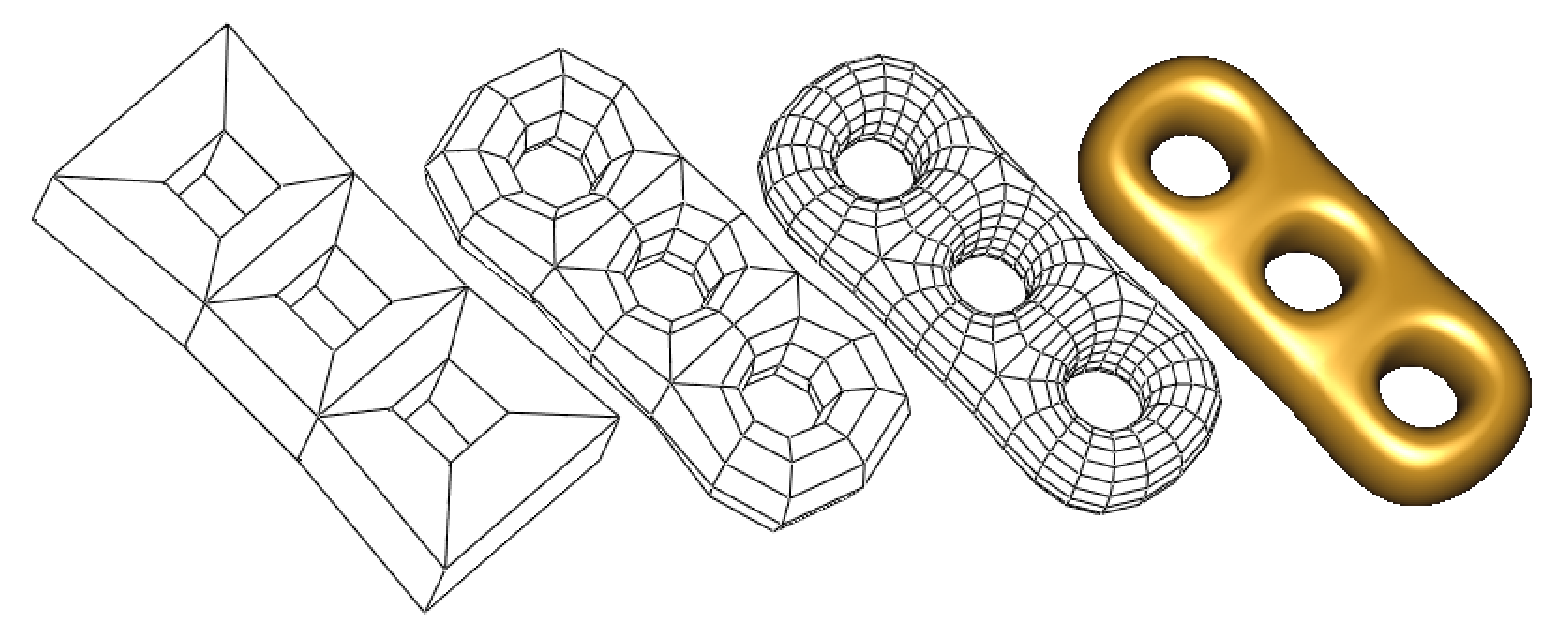
\includegraphics[width=12.0cm]{figs/teaser}}
    \caption{Snapshot taken from the tutorial application running
             on Windows. A polygon mesh is subdivided using the
             quad-triangle subdivision scheme~\cite{sl-qts-02}.}
    \label{fig:teaser}
\end{figure}
        

% targeted audience ?

The main targeted audience is a master or a Ph.D. student in computer
graphics or computational geometry, aiming at doing some research on
mesh processing algorithms. We hope this tutorial will convince the
reader~:

\begin{itemize}

\item 
not reinventing the wheel. Taking some time choosing the ``right
tool'' is often worth it. This may true, even for a short project;

\item 
using an optimized and robust library to ease the implementation and
obtain fast and robust results. This allows focusing on the elaborated
algorithm, not on the underlying data structure;

\item 
using generic programming to reuse existing data structures
and algorithms;

\item 
using a standard library in order to benefit from existing support and
discussion groups\footnote{see the cgal discuss list:
\href{http://www.cgal.org/user_support.html}
{http://www.cgal.org/user\_support.html.}}.

\end{itemize}               


% PREREQUISITES
\section{Prerequisites}

% C++ and generic programming

Before using CGAL, it is mandatory to be familiar with C++ and the
\italic{generic programming paradigm}. The latter features the notion
of C++ class templates and function templates, which is at the corner
stone of all features provided by CGAL.\\

% STL

An example illustrating generic programming is the Standard Template
Library (STL)~\cite{ms-stl-96}. Generality and flexibility is achieved
with a set of \italic{concepts}, where a concept is a well defined set
of requirements. One of them is the \italic{iterator} concept, which
allows both referring to an item and traversing a sequence of
items. Those items are stored in a data structure called
\italic{container} in STL. Another concept, so-called
\italic{circulator}, allows traversing some circular sequences. They
share most of the requirements with iterators, except the lack of
past-the-end position in the sequence. Since CGAL is strongly inspired
from the genericity of STL, it is important to become familiar with
its concepts before starting using it.

% HALFEDGE DATA STRUCTURE
\section{Halfedge data structure}

The specification of a polygon surface mesh consists of combinatorial
entities: vertices, edges, and faces, and numerical quantities:
attributes such as vertex positions, vertex normals, texture
coordinates, face colors, etc. The \italic{connectivity} describes the
incidences between elements and is implied by the topology of the
mesh. For example, two vertices or two faces are adjacent if there
exists an edge incident to both.\\

% definition

A \italic{halfedge data structure} is an edge-centered data structure
capable of maintaining incidence informations of vertices, edges and
faces, for example for planar maps, polyhedra, or other orientable,
two-dimensional surfaces embedded in arbitrary dimension. Each edge is
decomposed into two halfedges with opposite orientations. One incident
face and one incident vertex are stored in each halfedge. For each
face and each vertex, one incident halfedge is stored (see
Fig.\ref{fig:halfedge}).

% halfedge

\begin{figure}[htb]
    \centering{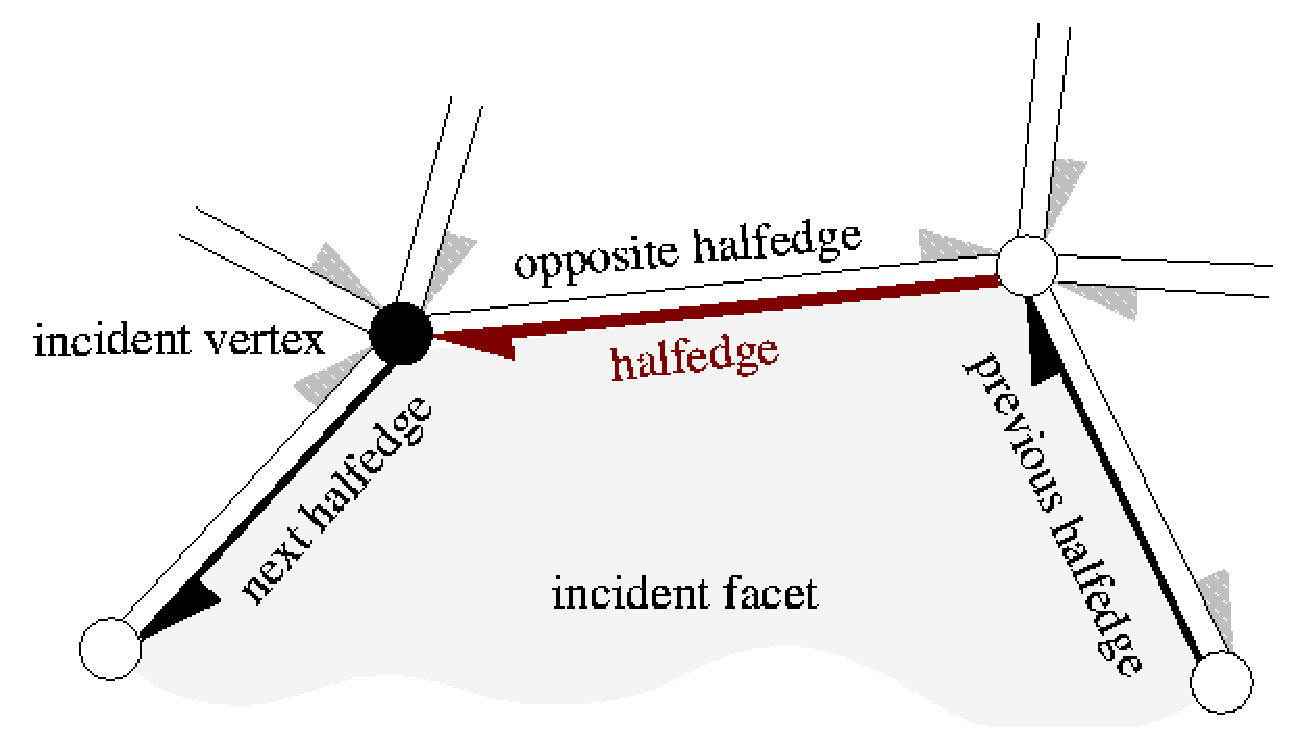
\includegraphics[width=7.0cm]{figs/halfedge}}
    \caption{One halfedge and its incident primitives.}
    \label{fig:halfedge}
\end{figure}
        
Notice that the halfedge data structure is only a combinatorial data
structure, geometric interpretation being added by classes built on
top of the halfedge data structure. On example is the class
\italic{CGAL::Polyhedron\_3} used in this tutorial. The 
halfedge data structure has been very successful for the design of
algorithms on meshes for several reasons:

\begin{itemize}

\item 
an edge-based data structure leads to a constant size structure,
contrary to face-based data structures with inevitable variable
topological structure when dealing with arbitrary vertex valence and
face degrees.

\item 
a halfedge encodes the orientation of an edge, facilitating the mesh
traversal.

\item 
navigation around each vertex by visiting all surrounding edges or
faces is made easy.

\item
each halfedge can be associated with a unique corner, that is a couple
$\{$face,vertex$\}$. The storage of attributes such as normals or
texture coordinates per corner (instead of per vertex) is thus
allowed.

\end{itemize}

% POLYHEDRON DATA STRUCTURE
\section{Polyhedron Data Structure}
\label{sec:polyhedron}

The class \verb+Polyhedron_3+ can represent polygon
meshes\footnote{\href{http://www.cgal.org/Manual/doc_html/basic_lib/Polyhedron_ref/Class_Polyhedron_3.html}{http://www.cgal.org}}.
Its underlying combinatorial component is based on the halfedge data
structure. As all CGAL geometric entities, its geometric component is
templated by the
\italic{kernel}\footnote{\href{http://www.CGAL.org/Manual/doc_html/frameset/fsKernel.html}{CGAL kernel}}.

\subsection{Declaration}

The simplest declaration of the polyhedron (without extended
primitives) consists of templating with a cartesian kernel and double
number precision:

{ \scriptsize
\begin{verbatim}
// instanciation of a polyhedron

#include <CGAL/Cartesian.h>
#include <CGAL/Polyhedron_3.h>

typedef CGAL::Cartesian<double>     kernel;
typedef CGAL::Polyhedron_3<kernel>  Polyhedron;

Polyhedron p;
\end{verbatim}}

\subsection{Extending primitives}

The polyhedron can be parameterized by a \italic{traits} class in
order to extend the vertex, halfedge and facet primitives. In this
tutorial all primitives (facets, halfedges and vertices) are
extended. The facet is extended with a normal and with a
general-purpose integer tag:

{ \scriptsize
\begin{verbatim}

template <class	Refs, class T, class P, class Norm>
class Enriched_facet : 
  public CGAL::HalfedgeDS_face_base<Refs, T>
{
  // tag
  int m_tag;

  // normal
  Norm m_normal;

public:

  // no  constructors to  repeat,  since  only
  // default constructor mandatory
  Enriched_facet()
  {
  }

  // tag
  const int&  tag()  {  return m_tag;  }
  void tag(const int& t)  {  m_tag  =  t; }

  // normal
  typedef  Norm Normal_3;
  Normal_3&  normal() { return  m_normal;  }
  const  Normal_3&  normal() const { return  m_normal;  }
};
\end{verbatim}}

The halfedge is extended with a general-purpose tag and a binary tag
to indicate wether it belongs to the control mesh or not. The latter
tag is used to superimpose the control mesh as shown in
Fig.\ref{fig:teaser}.

{ \scriptsize
\begin{verbatim}

template <class  Refs, class Tprev, class Tvertex, 
          class Tface, class Norm>
class Enriched_halfedge : public 
  CGAL::HalfedgeDS_halfedge_base<Refs,Tprev,Tvertex,Tface>
{
private:

  // tag
  int  m_tag; 

  // option  for control edge superimposing
  bool m_control_edge; 

public:

  // life  cycle
  Enriched_halfedge()
  {
    m_control_edge = true;
  }

  // tag
  const int& tag() const { return m_tag;  }
  int& tag() { return m_tag;  }
  void tag(const int& t)  {  m_tag  =  t; }

  // control edge  
  bool& control_edge()  { return m_control_edge; }
  const bool& control_edge()  const { return m_control_edge; }
  void control_edge(const bool& flag) { m_control_edge  =  flag;  }
};

\end{verbatim}}

The vertex is extended with a normal and a general-purpose integer
tag:

{ \scriptsize
\begin{verbatim}


template <class  Refs, class T, class P, class Norm>
class Enriched_vertex :  
  public CGAL::HalfedgeDS_vertex_base<Refs, T, P>
{
  // tag
  int  m_tag; 

  // normal
  Norm m_normal;

public:
  // life  cycle
  Enriched_vertex() {}
  // repeat  mandatory  constructors
  Enriched_vertex(const  P& pt)
    :  CGAL::HalfedgeDS_vertex_base<Refs, T,  P>(pt)
  {
  }

  // normal
  typedef  Norm Normal_3;
  Normal_3&  normal() { return  m_normal;  }
  const  Normal_3&  normal() const { return  m_normal;  }

  // tag
  int& tag() {  return m_tag;  }
  const int& tag() const {  return m_tag;  }
  void tag(const int& t)  {  m_tag  =  t; }
};

\end{verbatim}}



A redefined items class for the polyhedron uses the class wrapper
mechanism to embedd all three extended primitives within one unique
class.

{ \scriptsize
\begin{verbatim}

struct Enriched_items : public CGAL::Polyhedron_items_3
{
    // wrap  vertex
    template <class  Refs,  class  Traits>
    struct Vertex_wrapper
    {
        typedef  typename Traits::Point_3  Point;
        typedef  typename Traits::Vector_3  Normal;
        typedef  Enriched_vertex<Refs,
                          CGAL::Tag_true,
                          Point,
                          Normal>  Vertex;
    };

    // wrap  face
    template <class  Refs,  class  Traits>
    struct Face_wrapper
    {
        typedef  typename Traits::Point_3  Point;
        typedef  typename Traits::Vector_3  Normal;
        typedef  Enriched_facet<Refs,
                         CGAL::Tag_true,
                         Point,
                         Normal> Face;
    };

    // wrap  halfedge
    template <class  Refs,  class  Traits>
    struct Halfedge_wrapper
    {
        typedef  typename Traits::Vector_3  Normal;
        typedef  Enriched_halfedge<Refs,
                            CGAL::Tag_true,
                            CGAL::Tag_true,
                            CGAL::Tag_true,
                            Normal>  Halfedge;
    };
};
\end{verbatim}}

The trait class is then used for templating a polyhedron
\italic{Enriched\_polyhedron}:

{ \scriptsize
\begin{verbatim}

template <class  kernel,  class  items>
class  Enriched_polyhedron :
  public CGAL::Polyhedron_3<kernel,items>
{
  //...
};
\end{verbatim}}

The corresponding instanciation of an enriched polyhedron follows:

{ \scriptsize
\begin{verbatim}

#include <CGAL/Simple_cartesian.h>
#include "enriched_polyhedron.h"

typedef double number_type;
typedef CGAL::Simple_cartesian<number_type> kernel;

Enriched_polyhedron<kernel,Enriched_items> polyhedron;

\end{verbatim}}



\subsection{Iteration and Circulation}

The \italic{iterator} STL concept allows traversing a sequence of
items. This concept is applied to the primitives of a mesh, be they
halfedges, edges, vertices, facets or points. Notice that the order of
iteration is not dictated by any incidence relationship, contrary to
the circulator. The following example shows how to iterate on the mesh
vertices.

{ \scriptsize
\begin{verbatim}
Vertex_iterator iter;
for(iter = polyhedron.vertices_begin();
    iter != polyhedron.vertices_end();
    iter++)
{
  Vertex_handle hVertex = iter;
  // do something with hVertex
}
\end{verbatim}}

The \italic{circulator} STL concept allows traversing a circular
sequence of items. This concept is applied both inside facets and
around vertices. 

\paragraph{Circulating around a facet}
The facets being defined by the circular sequence of halfedges along
their boundary, this calls for a circulator around a facet. The
convention is that the halfedges are oriented counterclockwise around
facets as seen from the outside of the polyhedron (see
Fig.\ref{fig:stl_concept}, left).

{ \scriptsize
\begin{verbatim}
// circulate around hFacet
Halfedge_around_facet_circulator circ = hFacet->facet_begin();
Halfedge_around_facet_circulator end = circ;
CGAL_For_all(circ,end)
{
  Halfedge_handle hHalfedge = circ;
  // do something with hHalfedge
}
\end{verbatim}}

\paragraph{Circulating around a vertex}
The convention being that the halfedges are oriented counterclockwise
around facets as seen from the outside of the polyhedron, this implies
that the halfedges are oriented clockwise around the vertices (see
Fig.\ref{fig:stl_concept}, right).

{ \scriptsize
\begin{verbatim}
// circulate around hVertex
Halfedge_around_vertex_circulator circ = hVertex->vertex_begin();
Halfedge_around_vertex_circulator end = circ;
CGAL_For_all(circ,end)
{
  Halfedge_handle hHalfedge = circ;
  // do something with hHalfedge
}
\end{verbatim}}

% circulation inside a facet and around a vertex
\begin{figure}[htb]
    \centering{\includegraphics[width=7.0cm]{figs/stl_concepts}}
    \caption{Left: circulation around a facet (ccw).
             Right: circulation around a vertex (cw).}  
    \label{fig:stl_concept}
\end{figure}

\subsection{Mesh Editing}

The polyhedron provides a series of atomic operators to modify the
connectivity of the polyhedral surface:
\begin{itemize}
\item split or join of two facets,
\item split or join of two vertices,
\item split or join of two loops,
\item split of an edge.
\end{itemize}

Furthermore, more operators are provided to work with surfaces with
boundaries, to create or delete holes, add a facet to the border,
etc. We refere to the references manual for precise definitions and
illustratives figures\footnote{See
\href{http://www.cgal.org/Manual/doc_html/basic_lib/Polyhedron/Chapter_main.html}{Euler 
operators}}.

\subsection{Incremental Builder}
\label{sec:builder}

The utility class \verb+Polyhedron_incremental_builder_3+ helps in
creating polyhedral surfaces from a list of points followed by a list
of facets that are represented as indices into the point list. This is
particularly useful for implementing file reader for common file
formats. In Section~\ref{sec:subdivision_builder}, we use the
incremental builder to implement the quad-triangle subdivision
scheme.\\

In the following example, the incremental builder is used to create a
simple triangle. \verb+Build_triangle+ is such a function object
derived from \verb+Modifier_base<HalfedgeDS>+. The
\verb+delegate()+ member function of the polyhedron accepts this function
object and calls its \verb+operator()+ with a reference to its
internally used halfedge data structure. Thus, this member function in
\verb+Build_triangle+ can create the triangle in the 
halfedge data structure.

{ \scriptsize
\begin{verbatim}
// examples/Polyhedron/polyhedron_prog_incr_builder.C

#include <CGAL/Cartesian.h>
#include <CGAL/Polyhedron_incremental_builder_3.h>
#include <CGAL/Polyhedron_3.h>

// A modifier creating a triangle with 
// the incremental builder.

template <class HDS>
class Build_triangle
  : public CGAL::Modifier_base<HDS> 
{
public:
  Build_triangle() {}

  void operator()(HDS& hds) 
  {
    // Postcondition: `hds' is a valid polyhedral surface.
    CGAL::Polyhedron_incremental_builder_3<HDS> B(hds, true);
    B.begin_surface(3, 1, 6);
    typedef typename HDS::Vertex   Vertex;
    typedef typename Vertex::Point Point;
    B.add_vertex(Point(0, 0, 0));
    B.add_vertex(Point(1, 0, 0));
    B.add_vertex(Point(0, 1, 0));
    B.begin_facet();
    B.add_vertex_to_facet(0);
    B.add_vertex_to_facet(1);
    B.add_vertex_to_facet(2);
    B.end_facet();
    B.end_surface();
  }
};

typedef CGAL::Cartesian<double>     Kernel;
typedef CGAL::Polyhedron_3<Kernel>  Polyhedron;
typedef Polyhedron::HalfedgeDS      HalfedgeDS;

Polyhedron P;
Build_triangle<HalfedgeDS> triangle;
P.delegate(triangle);
CGAL_assertion(P.is_triangle(P.halfedges_begin()));

\end{verbatim}}

% SUBDIVISION SURFACES
\section{Subdivision Surfaces}

A subdivision surface is the limit surface resulting from the
application of a \italic{subdivision scheme} to a control polyhedron
(see Fig.\ref{fig:teaser}). During this process the polygon base
mesh is recursively subdivided and the mesh geometry is progressively
modified according to subdivision rules. A subdivision scheme is
characterized by a refinement operator that acts on the connectivity
by subdividing the mesh, and by a smoothing operator that modifies the
geometry. 

Figure. \ref{fig:RefSchemes} introduces several refinement schemes in
practice. Some general properties of these refinement schemes are
\italic{regular pattern}, \italic{rotationally symmetric} and well
\italic{defined footprint} of each vertex in the
range. Figure. \ref{fig:PQQMap} demonstrates the functional map from
the footprint in the domain mesh to the vertex in the range mesh of
the primal quadrilateral quadrisection scheme. The geometry rules of a
specific refinement scheme is hence defined according to the
corresponding functional maps.

\begin{figure}
  \centering
  \subfigure[Primal quadrilateral quadrisection.] {
    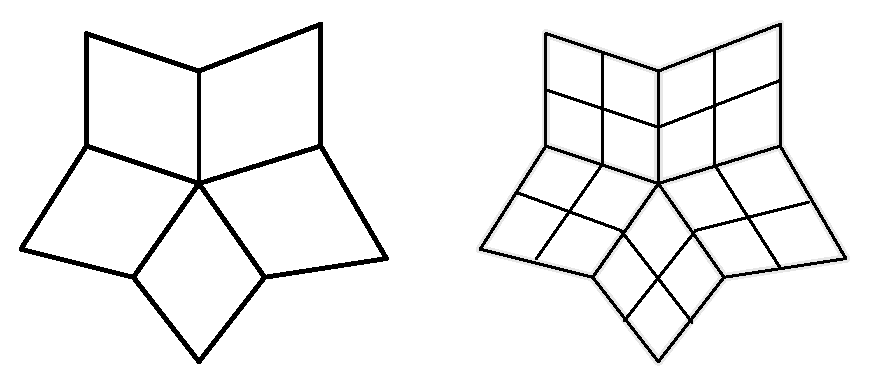
\includegraphics[width=2.5in]{pfigs/PQQRef.eps}
  }
  \subfigure[Primal triangle quadrisection.] {
    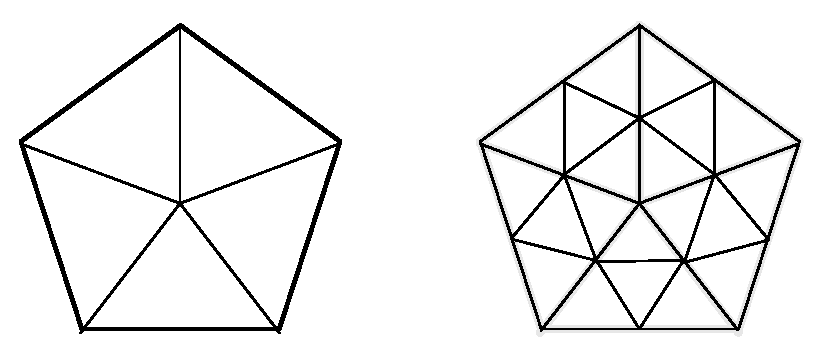
\includegraphics[width=2.5in]{pfigs/PTQRef.eps}
  }
  \subfigure[Dual quadrilateral quadrisection.] {
    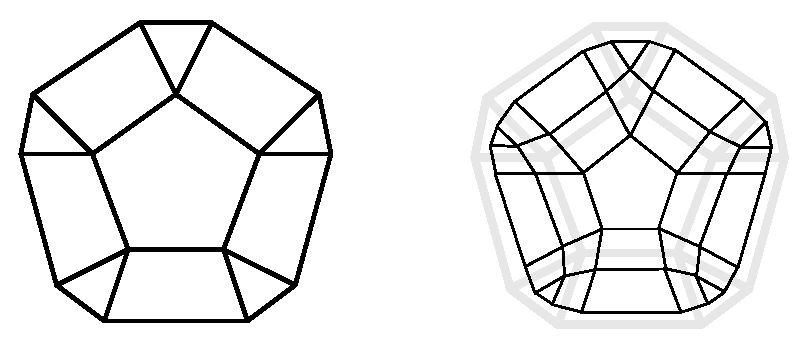
\includegraphics[width=2.5in]{pfigs/DQQRef.eps}
  }
  \caption{Refinement schemes. (Left) indicates the domain mesh.
  (Right) indicates the range mesh. }
  \label{fig:RefSchemes}
\end{figure}

\begin{figure}
  \centering
  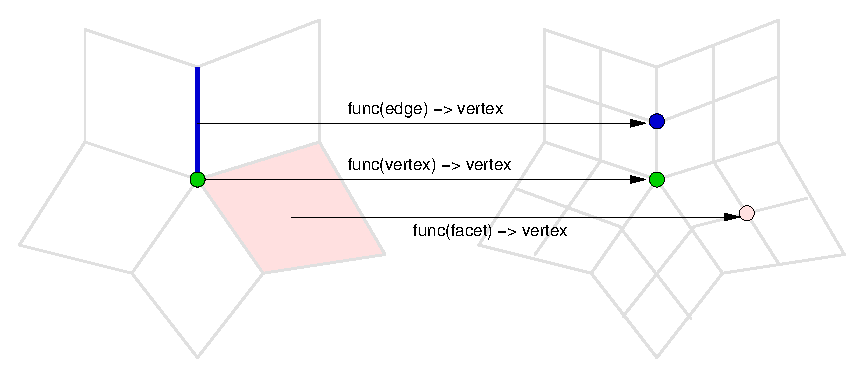
\includegraphics[width=3.0in]{pfigs/PQQRefMap.eps}\\
  \caption{The correspondence of the domain footprint and the 
           range vertex of the PQQ schemes}
  \label{fig:PQQMap}
\end{figure}

Any implementation of a subdivision scheme contains two major
components: \italic{refinement scheme} and \italic{geometry rules}.
Refinement schemes are defined by the 
\italic{uniform connectivity reconfiguration} of the source 
mesh (the domain) to the target mesh (the range). The geometry rules,
providing certain surface properties, e.g the smoothness, are the
mapping functions of the \italic{footprints} in the domain mesh to the
\italic{vertices} in the range mesh. Any subdivision in practice can
be defined as a legal combination of a refinement scheme and the
geometry rules. Based on the paradigm of the
\italic{policy-based design} \cite{a-rotm-02}, the combination can be
designed as the \italic{host function} (the refinement function)
templated with the \italic{policy class} (the geometry rules).

\subsection{$\sqrt{3}$-Subdivision using Euler Operators}

\label{sec:subdivision_euler}

The $\sqrt{3}$ subdivision scheme was introduced by
Kobbelt~\cite{k-sqrt3-00}. It takes as input a triangle mesh and
subdivide each facet into three triangles by splitting it at its
centroid. Next, all edges of the initial mesh are flipped so that they
join two adjacent centroids. Finally, each initial vertex is replaced
by a barycentric combination of its neighbors. An example of one step
of the $\sqrt{3}$ subdivision scheme is shown in
Fig.\ref{fig:sqrt3_basic}, and an example of several steps is shown in
Fig.\ref{fig:sqrt3}.

% sqrt3 subdivision (basic)

\begin{figure}[htb]
    \centering{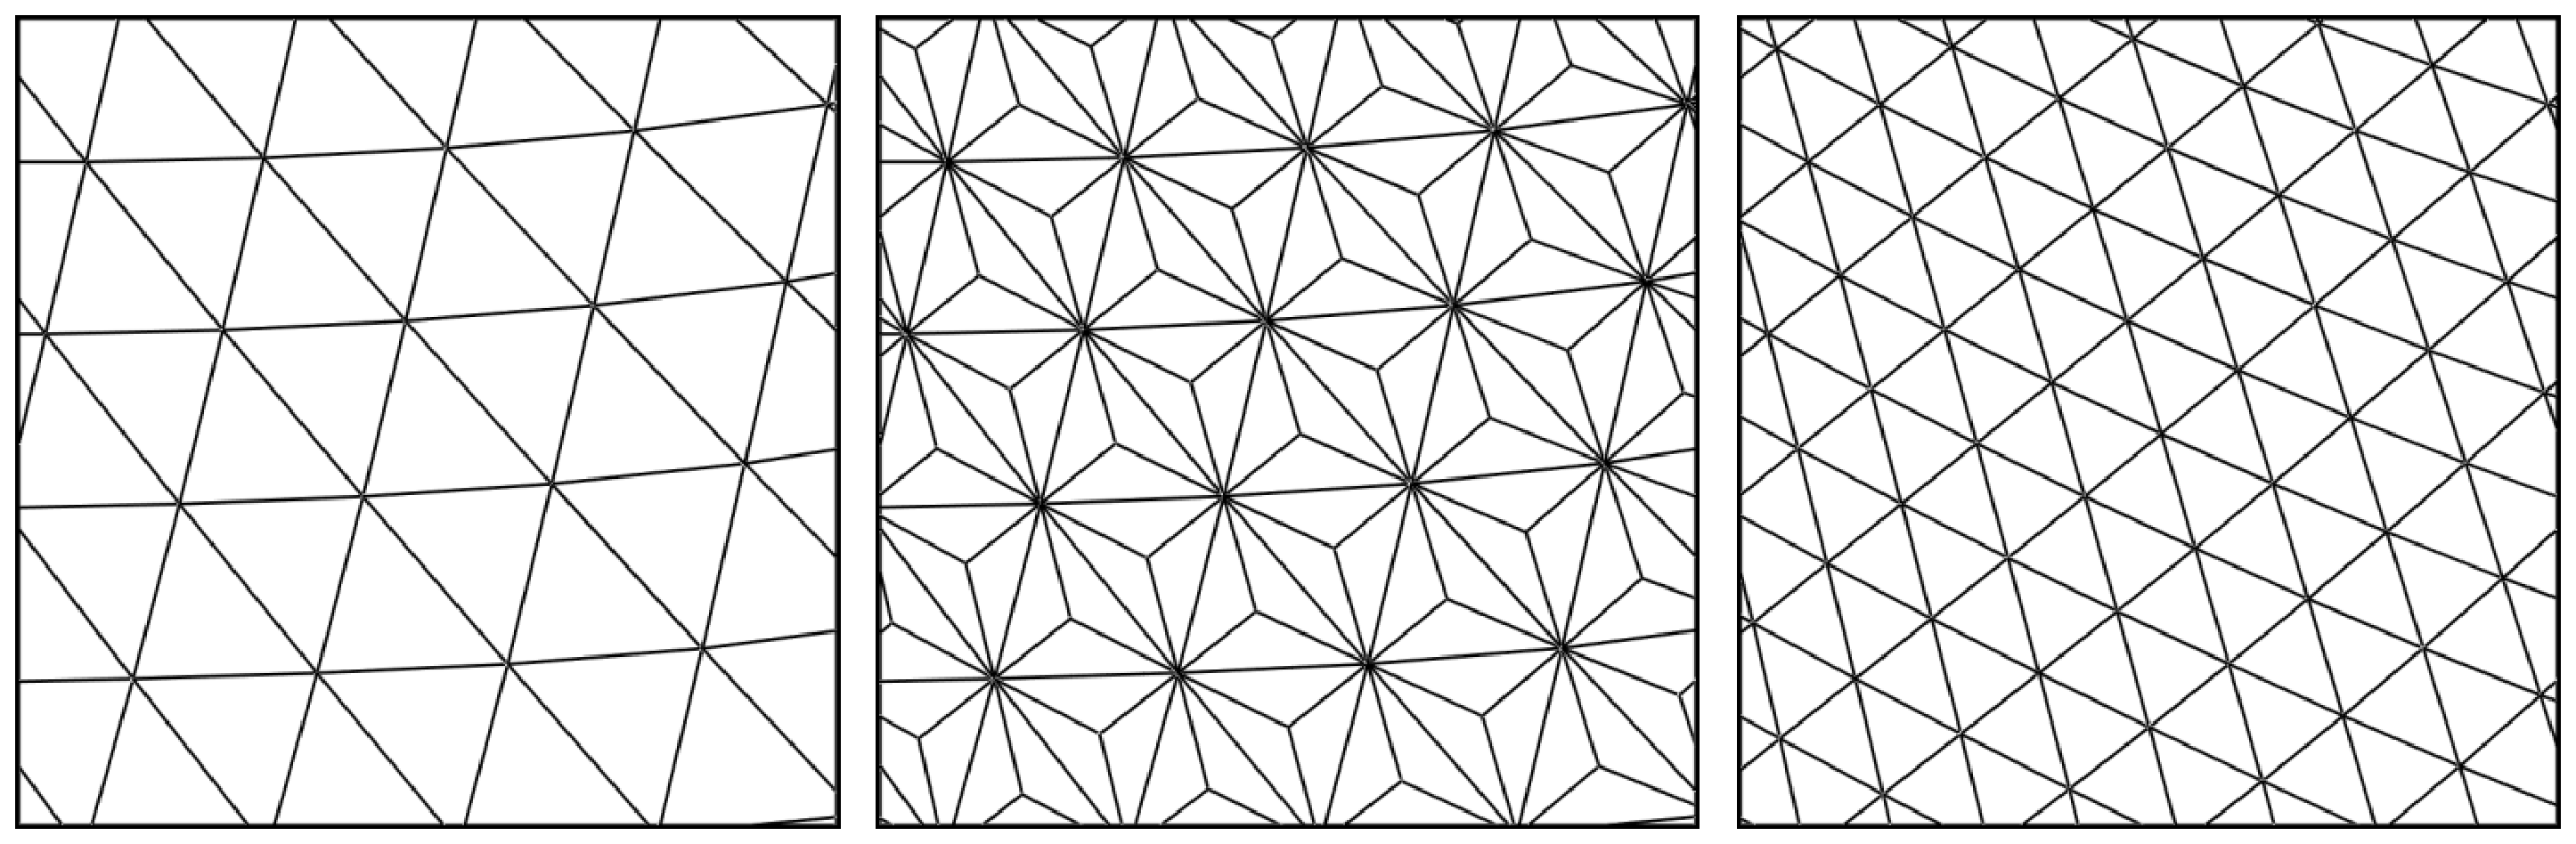
\includegraphics[width=10.0cm]{figs/sqrt3_basic}}
    \caption{The $\sqrt{3}$-Subdivision scheme is decomposed as
             a set of Euler operators: face splits and edge flips.}
    \label{fig:sqrt3_basic}
\end{figure}

{ 

\scriptsize
\begin{verbatim}



\end{verbatim}
}

% sqrt3 subdivision 

\begin{figure}[htb]
    \centering{\includegraphics[width=10.0cm]{figs/sqrt3}}
    \caption{$\sqrt{3}$-Subdivision of the mannequin mesh.}
    \label{fig:sqrt3}
\end{figure}


\subsection{Quad-triangle Subdivision using Incremental Builder}

\label{sec:subdivision_builder}

The quad-triangle subdivision scheme was introduced by
Levin~\cite{l-pg-03}, then Stam and Loop~\cite{sl-qts-02}. It applies
to polygon meshes and basically features Loop subdivision on triangles
and Catmull-Clark subdivision on polygons of the control mesh (see
Fig.\ref{fig:quad-triangle}). After one iteration of subdivision the
subdivided model is only composed of triangles and quads. A simple
solution for implementing such a scheme is to use the
\italic{incremental builder} concept featured by CGAL 
Polyhedron (see Section~\ref{sec:builder}).


% quad-triangle subdivision scheme

\begin{figure}[htb]
    \centering{\includegraphics[width=10.0cm]{figs/quad-triangle}}
    \caption{Quad-triangle subdivision scheme.}
    \label{fig:quad-triangle}
\end{figure}

Subdivision engine

{ \scriptsize
\begin{verbatim}

#include "enriched_polyhedron.h"
#include "builder.h"

template <class HDS,class Polyhedron,class kernel>
class CModifierQuadTriangle : public CGAL::Modifier_base<HDS>
{
private:

  typedef ...

  Polyhedron *m_pMesh;

public:

  // life cycle
  CModifierQuadTriangle(Polyhedron *pMesh)
  {
    CGAL_assertion(pMesh != NULL);
    m_pMesh = pMesh;
  }
  ~CModifierQuadTriangle() {}

  // subdivision
  void operator()( HDS& hds)
  {
    builder B(hds,true);
    B.begin_surface(3,1,6);
      add_vertices(B);
      add_facets(B);
    B.end_surface();
  }

private:

  // ... 
  // for the complete implementation of the subdivision, 
  // readers should refer to the accompanied source codes of 
  // this tutorial.
  
};
\end{verbatim}}

{ \scriptsize
\begin{verbatim}
template <class Polyhedron,class kernel>
class CSubdivider_quad_triangle
{
public:
    typedef typename Polyhedron::HalfedgeDS HalfedgeDS;

public:
  // life cycle
  CSubdivider_quad_triangle() {}
  ~CSubdivider_quad_triangle() {}

public:
  void subdivide(Polyhedron &OriginalMesh,
                 Polyhedron &NewMesh,
                 bool smooth_boundary = true)
  {
    CModifierQuadTriangle<HalfedgeDS,Polyhedron,kernel> 
      builder(&OriginalMesh);

    // delegate construction 
    NewMesh.delegate(builder);

    // smooth
    builder.smooth(&NewMesh,smooth_boundary);
  }
};
\end{verbatim}}

% SurfLab

\subsection{Subdivision using a rule template}

\label{sec:subdivision_rule}

We use Catmull-Clark (CC) subdivision as our first example (see
Figure~\ref{fig:cc}). CC subdivision can be defined as the combination
of the primal quadrilateral quadrisection (PQQ) scheme and the
Catmull-Clark geometry rules.

{\scriptsize
\begin{verbatim}
template <class Polyhedron, template <class> Rule>
void PrimalQuadQuadralize(Polyhedron& p, Rule<Polyhedron>& r) { ...}

template <class Polyhedron>
void CCSubdivision(Polyhedron& p) { 
  PrimalQuadQuadralize(p, CatmullClarkRule<Polyhedron>());
}
\end{verbatim}
}

For meshes based on PQQ scheme, the footprints of the range vertices
each corresponds to a topology primitive, i.e. vertex, edge or facet,
in the domain (see Figure. \ref{fig:PQQMap}).  The policy class hence
needs to provide the policy functions in each case.

{ \scriptsize
\begin{verbatim}
template <class P> class CatmullClarkRule 
{
public:
  typedef P                                    Polyhedron;
  typedef typename Polyhedron::Vertex_handle   Vertex_handle;
  typedef typename Polyhedron::Halfedge_handle Halfedge_handle;
  typedef typename Polyhedron::Facet_handle    Facet_handle;

  void face_vertex_rule(Facet_handle domain_f,    Vertex_handle range_v);
  void edge_vertex_rule(Halfedge_handle domain_e, Vertex_handle range_v);
  void vertex_vertex_rule(Vertex_handle domain_v, Vertex_handle range_v);
};
\end{verbatim}
}

Each policy function has two input parameters: the domain primitive
and the range vertex. The footprint, defined as the vertices set of
the 1-distance neighbors of the corresponding domain primitive, is
passed as the handle of the primitive. Empolying the incidental
function of the halfedge data structure, the policy designer works on
the simple view of the \italic{local} mesh corresponding to the
footprint. Following codes demonstrate the facet-vertex case.

{\scriptsize
\begin{verbatim}
void facet_vertex_rule(Facet_handle domain_f, Vertex_handle& range_v) 
{
  typedef typename Polyhedron::Point_3 Point;

  Halfedge_around_facet_circulator hcir = domain_f->facet_begin();
  Halfedge_around_facet_circulator hcir_end = hcir;
  range_v->point() = Point(0,0,0);
  do 
    range_v->point() += hcir->vertex()->point();
  while (++hcir != hcir_end);

  range_v->point() /= circulator_size(hcir);
}
\end{verbatim}
}

% Catmull-Clark subdivision

\begin{figure}[htb]
    \centering{\includegraphics[width=10.0cm]{figs/subdivision}}
    \caption{Catmull-Clark subdivision of a quadrilateral control mesh.}  
    \label{fig:cc}
\end{figure}

Loop subdivision uses similar refinement scheme to PQQ scheme except
that it works on the triangle mesh. Hence the footprints of Loop
scheme are same as the CC scheme but without the facet-vertex case.

{\scriptsize
\begin{verbatim}
PrimalTriangleQuadralize(p, LoopRule<Polyhedron>());

template <class Polyhedron>
void LoopSubdivision(Polyhedron& p) 
{ 
  PrimalTriangleQuadralize(p, LoopRule<Polyhedron>());
}

template <class P> class LoopRule 
{
public:
  typedef ...

  void edge_vertex_rule(Halfedge_handle domain_e, Vertex_handle range_v);
  void vertex_vertex_rule(Vertex_handle domain_v, Vertex_handle range_v);
};
\end{verbatim}
}

Doo-Sabin (DS) subdivision is fundamentally different from the primal
subdivision schemes in the aspect of the footprints. As showed in
Figure \ref{fig:PQQMap}, each range vertex corresponds to a
\italic{corner} in the domain mesh. The footprint of the range vertex
is the facet containing the corner.

\begin{figure}
  \centering
  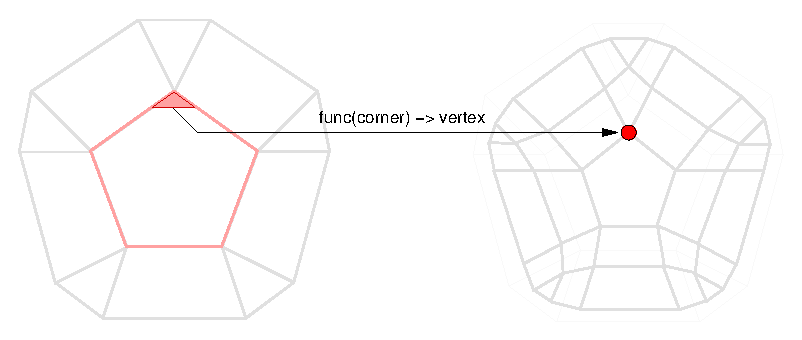
\includegraphics[width=2.5in]{pfigs/DQQRefMap.eps}
  \caption{The correspondence of the domain footprint and the 
           range vertex of the DQQ schemes.}
  \label{fig:DQQMap}
\end{figure}


{\scriptsize
\begin{verbatim}
DualQuadQuadralize(p, DooSabinRule<Polyhedron>());

template <class Polyhedron>
void DSSubdivision(Polyhedron& p) 
{ 
  DualQuadQuadralize(p, DooSabinRule<Polyhedron>());
}

template <class P> class DooSabinRule 
{
public:
  typedef ...

  void corner_vertex_rule(Halfedge_handle domain_e, Vertex_handle range_v);
};
\end{verbatim}
}

The only policy function for the DS subdivision has the halfedge
pointing to the corner as the domain parameter. A demo of policy
function for the regular facet, i.e. the quadrilateral facet, is
listed in the following codes.

{\scriptsize
\begin{verbatim}
void corner_vertex__rule(Halfedge_handle domain_e, Vertex_handle range_v) 
{
  range_v->point() = Point(0,0,0);

  range_v->point() = domain_e->vertex()->point() * 9 + 
                    (domain_e->next()->vertex()->point() +
                     domain_e->pre()->vertex()->point()) * 3 +
		     domain_e->next()->next()->vertex()->point();
  
  range_v->point() /= 16.0;
}
\end{verbatim}
}

For the complete implementation of the subdivision, readers should
refer to the accompanied source codes of this tutorial.

% APPLICATION DEMO
\section{Application demo}

List of features, snapshots (todo).

\subsection{Compiling on Windows}



(todo)

% REFERENCES
\bibliographystyle{alpha}
\bibliography{tutorial}


\end{document}
